\documentclass{report}
\usepackage{cite}
\usepackage{titlesec}
\usepackage{amsmath}
\usepackage[english]{babel}
\usepackage{caption}
\usepackage{multirow}
\usepackage{tikz}
\usepackage{amsmath}
\usepackage{amssymb}
\usetikzlibrary{calc}
\usetikzlibrary{arrows}
\usepackage{pgfplots}
\captionsetup[figure]{font=small}	
\captionsetup[table]{font=footnotesize}
\newcommand{\R}{\mathbb{R}}
\usepackage{float}
\tolerance=1
\emergencystretch=\maxdimen
\hyphenpenalty=10000
\hbadness=10000
\usepackage{array}
\usepackage[margin=1.5in]{geometry}
\usepackage{mathtools}

\begin{document}


\begin{titlepage}
\begin{center}
\vspace*{0.8cm}
\begin{figure}[H]
\centering

\includegraphics[width=0.4\textwidth]{logo_uni}
\end{figure}
\LARGE{\textsc{University of Padua}}\\
\vspace*{0.1cm}
\Large{\textsc{Department of Information Engineering}}\\
\vspace*{1.8cm}
\Large{\textsc{Information Security Report}}\\
\vspace*{0.1cm}
\Large{\textsc{Team Blue}}\\
\vspace*{0.8cm}
\huge{\textbf{Implementation and weakness evaluatation of a challenge-response scheme for entity authentication}}\\
\vspace*{1cm}
\end{center}
\large{\textit{Authors:}}
\hfill
\large{\textit{Teacher:}} \\
\large{Sara \textsc{Bardi}}
\hfill
\large{Nicola \textsc{Laurenti}}\\
\large{Simone \textsc{Favaro}}\\
\large{Alessandro \textsc{Rizzo}}\\
\large{Enrico \textsc{Tiozzo}}\\

\begin{center}
\large{20th December 2020}\\
\end{center}
\end{titlepage}
\pagebreak

\setcounter{page}{1}
\pagenumbering{arabic}






\chapter*{Tasks implementation}

\section*{Task 1}
\subsection*{Protocol implementation}
{\tt task1.py} contains the entity authentication scheme. The main idea behind our implementation is using two different data structures in order for $A$ and $B$ to store the messages and the relevant variables they exchange during the communication steps. In order to accomplish that, we initialize two different python dictionaries containing the following keys: \textit{key, challenge, n\_counter, id\_A, u2, r}.\\
Moreover, the script is design in such a way that the setup and each other protocol step is implemeted by a different method:
\begin{itemize}

\item {\tt setup(n,lk)} initializes the {\tt n} value, the key length {\tt lk} and the id of $A$ {\tt id\_A}, then it generates a random binary key which is stored in $A$'s and $B$'s dictionaries. Finally, {\tt n} is stores in $B$ and {\tt id\_A} in $A$. It outputs {\tt id\_A} and the key.

\item {\tt step1()} simulates the sending of $u_1 = id\_A$ from $A$ to $B$. It outputs $u_1$,

\item{\tt  step2(lc)} first updates the {\tt n} value in $B$, then uses the initialization of the challenge length {\tt lc} to generate a random binary challenge. Finally the method simulates the sending of $u_2 = (c, n)$ from $B$ to $A$. It outputs $u_2$,

\item {\tt step3()} uses the util function {\tt r\_calc} which follows step 3 instructions in order to compute $u_3=r$. Then it simulates the sending of $u_3$ from $A$ to $B$. It outputs $r$.

\item {\tt step4()} let $B$ compute $\hat{r}$ using the same {\tt r\_calc} method. It outputs the $\hat{r}$ value.

\end{itemize}
 
 
 
\subsection*{Protocol implementation}
Concerning the computational complexity of the protocol implementation, the following plot represents the execution time for different values of key length (from 1 bit to 10000 bits). Each curve of the same color is composed by the raw data sampled by the {\tt time\_protocol} method (which uses the {\tt time} function to measure the correponding executions) and the line interpolation of the raw data. This is repeated for three different values of {\tt lc}: 8, 256 and 1024.   

\begin{figure}[H]
\centering
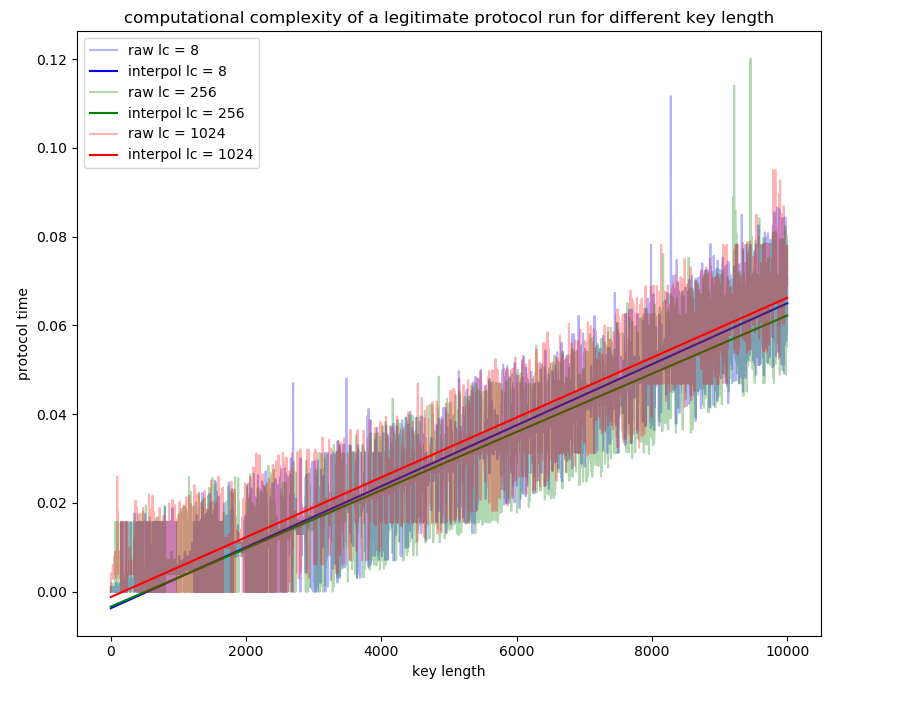
\includegraphics[width=1\textwidth]{plot1}
\end{figure}	

From the plot analysis, follows these observations:
\begin{itemize}

\item the curves follow a linear trend, to it is safe to say that the execution time is linear with respect to the key length.

\item even if the noise is relatively high on this scale, we think that it does not depend on {\tt lk}, but on the machine computations; and that for bigger key values it becomes more and more insignificant with respect to the execution time. 

\item  we observe that for similar {\tt lc} values the interpolation lines are almost congruent (actually, because of the randomness nature and the bit impact of the noise, the {\tt lc}=8 and {\tt lc}=256 curves have the same biases and the former has even a steeper slope).\\
However, we notice that for {\tt lc}=1024, the bias is higher than the other two curves: this means that even the {\tt lc} has influence on the execution time, since all time measures are higher than the corresponding ones with a less {\tt lc} value. 

\end{itemize}
 
 
 
 
 
 
 
 




\section*{Task 2 - First attack implementation}





\section*{Task 3 - Second attack implementation}





\end{document}

